\section{Deriving a functional approach}
%2 main points from Henrik: 1.: try to stick to synchronous updates because this is how the real world works. 2.: get rid of globally shared mutable state as it complicates things extremely with reasoning
%clear conceptual formal model of what agents are and then structure my implementation around it

In this section we will derive a functional approach for implementing an agent-based simulation of the SIR model. We will start out with a very naive approach and show its limitations which can be overcome by bringing in FRP. Then in three steps we will add more concepts and generalisations, ending up at the final approach which utilises monadic stream functions (MSF) \cite{perez_functional_2016}, a generalisation of FRP.
Although we presented a high-level agent-based approach to the SIR model in the previous section, which focused only on the states and the transitions, we haven't talked about technical implementation details on how to actually implement such a state-machine. In these steps we will ultimately present four different approaches on how to implement these states and transitions. Although all result \textit{on average} in the same dynamics, not all of them are equally expressive and testable.

\subsection{Step I: Naive beginnings}
In our first step we start with modelling the states of the agents for which we simply use an Algebraic Data Type (ADT):

\begin{minted}[fontsize=\footnotesize]{haskell}
data SIRState = Susceptible | Infected | Recovered
\end{minted}

Also agents are ill for some duration meaning we need to keep track when a potentially infected agent recovers. Also as previously mentioned, a simulation is stepped in discrete or continuous time-steps thus we introduce a notion of \textit{time} and $\Delta t$ by defining:

\begin{minted}[fontsize=\footnotesize]{haskell}
type Time      = Double
type TimeDelta = Double
\end{minted}

Now we can represent every agent simply as a tuple of its SIR-state and its potential recovery time. We hold all our agents simply in a list and define helper functions:
\begin{minted}[fontsize=\footnotesize]{haskell}
type SIRAgent = (SIRState, Time)
type Agents   = [SIRAgent]

is :: SIRState -> SIRAgent -> Bool
is s (s',_) = s == s'

susceptible :: SIRAgent
susceptible = (Susceptible, 0)

infected :: Time -> SIRAgent
infected t = (Infected, t)

recovered :: SIRAgent
recovered = (Recovered, 0)
\end{minted}

Next we need to think about how to actually step our simulation. For this we define a function which simply steps our simulation with a fixed $\Delta t$ until a given time $t$ where in each step the agents are processed and the output is fed back into the next step.
TODO: need a much better explanation and maybe split up into more steps?
As already mentioned in previous sections, the agent-based implementation of the SIR model is inherently stochastic which means we need access to a random-number generator. We decided to use the Rand Monad at this point as threading a generator through the simulation and the agents is very cumbersome. Thus our simulation stepping runs in the Rand Monad:

\begin{minted}[fontsize=\footnotesize]{haskell}
runSimulation :: RandomGen g 
              => Time 
              -> TimeDelta 
              -> Agents 
              -> Rand g [Agents]
runSimulation tEnd dt as = runSimulationAux 0 dt as []
  where
    runSimulationAux :: RandomGen g 
                     => Time 
                     -> TimeDelta 
                     -> Agents 
                     -> [Agents] 
                     -> Rand g [Agents]
    runSimulationAux t dt as acc
      | t >= tEnd = return $ reverse (as : acc)
      | otherwise = do
        as' <- stepSimulation dt as 
        runSimulationAux (t + dt) dt as' (as : acc)

stepSimulation :: RandomGen g => TimeDelta -> Agents -> Rand g Agents
stepSimulation dt as = mapM (processAgent dt as) as
\end{minted}

Now we can implement the behaviour of an individual agent. First we need to distinguish between the agents SIR-states:

\begin{minted}[fontsize=\footnotesize]{haskell}
processAgent :: RandomGen g 
             => TimeDelta 
             -> Agents 
             -> SIRAgent 
             -> Rand g SIRAgent
processAgent _  as    (Susceptible, _) = susceptibleAgent as
processAgent dt _   a@(Infected   , _) = return $ infectedAgent dt a
processAgent _  _   a@(Recovered  , _) = return a
\end{minted}

An agent gets fed all the agents states so it can draw random contacts. Note that this includes also the agent itself thus we would need to omit the agent itself to prevent making contact with itself. We decided against that as it complicates the solution and for larger numbers of agent population the probability for an agent to make contact with itself is so small that it can be neglected.

From our implementation it becomes apparent that only the behaviour of a susceptible agent involves randomness and that a recovered agent is simply a sink: it does nothing - its state stays constant.

Lets look how we can implement the behaviour of a susceptible agent. It simply makes contact on average with a number of other agents and gets infected with a given probability if an agent it has contact with is infected.
When the agent gets infected it calculates also its time of recovery by drawing a random number from the exponential distribution meaning it is ill on average for illnessDuration.

\begin{minted}[fontsize=\footnotesize]{haskell}
susceptibleAgent :: RandomGen g => Agents -> Rand g SIRAgent
susceptibleAgent as = do
    rc <- randomExpM (1 / contactRate)
    cs <- doTimes (floor rc) (makeContact as)
    if elem True cs
      then infect
      else return susceptible

  where
    makeContact :: RandomGen g => Agents -> Rand g Bool
    makeContact as = do
      randContact <- randomElem as
      if (is Infected randContact)
        then randomBoolM infectivity
        else return False

    infect :: RandomGen g => Rand g SIRAgent
    infect = do
      randIllDur  <- randomExpM (1 / illnessDuration)
      return  infected randIllDur
\end{minted}

The infected agent is trivial. It simply recovers after the given illness duration which is implemented as follows:

\begin{minted}[fontsize=\footnotesize]{haskell}
infectedAgent :: TimeDelta -> SIRAgent -> SIRAgent
infectedAgent dt (_, t) 
    | t' <= 0   = recovered
    | otherwise = infected t'
  where
    t' = t - dt  
\end{minted}

\subsubsection{Results}
We run the simulation for $t = 150$ time-units with a fixed $\Delta t = 1.0$. With increasing number of agents the dynamics approach the one of the SD simulation. TODO: add pictures

Reflecting on our first naive approach we can conclude that it already introduced the most fundamental concepts of ABS
\begin{itemize}
	\item Time - the simulation occurs over virtual time which is modelled explicitly divided into \textit{fixed} $\Delta t$ where at each the agents are executed.
	\item Agents - we implement each agent as an individual behaviour which depends on the agents state.
	\item Feedback - the output state of the agent in the current time-step $t$ is the input state for the next time-step $t+1$.
	\item Environment - as environment we implicitly assume a fully-connected network where every agent 'knows' every other agents, including itself and thus can make contact with every other agent (including itself).
	\item Stochasticity - its an inherently stochastic simulation, which is indicated by the Rand Monadic type.
	\item Deterministic - repeated runs with the same initial random-number generator result in same dynamics. This may not come as a surprise but in Haskell we can guarantee that property statically already at compile time because our simulation runs in the Rand monad and NOT in the IO Monad. This guarantees that no external, uncontrollable sources of randomness can interfere with the simulation.
	\item Dynamics - it works as expected: with increasing number of agents our solution approaches the SD dynamics 
\end{itemize}

Nonentheless our approach has also weaknesses and dangers:
\begin{enumerate}
	\item $\Delta t$ is passed explicitly as argument to the agent and needs to be dealt with explicitly. It seems to be not very elegant and a potential source of errors - can we do better and find a more elegant solution? 
	\item The way our agents are represented is not very elegant: the state of the agent is explicitly encoded in an ADT and when processing the agent the function needs always first distinguish between the states. Can we express it in a more implicit, functional way?
	\item The states of all agents of the current step are fed back into every agent in the next step so that an agent can pick its contacts. Although agents cannot change the states, this reveals too much information e.g. the illness duration is of no interest to the other agents. Although we could just feed in the SIRStates without the illness duration, the problem is more of conceptual nature: it should be the agent which decides to whom it reveals which information.
\end{enumerate}

We move now to the next step in which we will address points 1 and 2, point 3 will be solved in step 3.

\subsection{Adding Functional Reactive Programming}
\label{sec:step2_frp}
As shown in the first step, the need to handle $\Delta t$ explicitly can be quite messy, is inelegant and a potential source of errors, also the explicit handling of the state of an agent and its behavioural function is not very functional. We can solve both these weaknesses by switching to the functional reactive programming (FRP) paradigm, because it allows to express systems with discrete and continuous time-semantics. In this step we are focusing on arrowized FRP using the library Yampa. In it, time is handled implicit and cannot be messed with and the whole system is built on the concept of signal-functions (SF). A signal-function is basically a continuation which allows then to capture state using closures. Both these fundamental features allow us to tackle the weaknesses of our first step and push our approach further towards a truly functional approach.

\subsubsection{Short introduction to Yampa}
TODO: introduce FRP / Yampa here

\subsubsection{Implementation}
We start by defining our agents now as a signal-function which receives the states of all agents as input and outputs the state of the agent:

\begin{minted}[fontsize=\footnotesize]{haskell}
type SIRAgent = SF [SIRState] SIRState 
\end{minted}

Now we can define the behaviour of an agent to be the following:

\begin{minted}[fontsize=\footnotesize]{haskell}
sirAgent :: RandomGen g => g -> SIRState -> SIRAgent
sirAgent g Susceptible = susceptibleAgent g
sirAgent g Infected    = infectedAgent g
sirAgent _ Recovered   = recoveredAgent
\end{minted}

Depending on the initial state we return one of three functions. Most notably is the difference that we are now passing a random-number generator instead of running in the Random Monad because signal-functions as implemented in Yampa are not capable of being monadic. We see that the recovered agent ignores the random-number generator which is in accordance with the implementation in the previous step where it acts as a sink which returns constantly the same state:

\begin{minted}[fontsize=\footnotesize]{haskell}
recoveredAgent :: SIRAgent
recoveredAgent = arr (const Recovered)
\end{minted}

The implementation of a susceptible agent in FRP is a bit more involved but much more expressive and elegant:

\begin{minted}[fontsize=\footnotesize]{haskell}
susceptibleAgent :: RandomGen g => g -> SIRAgent
susceptibleAgent g = switch (susceptible g) (const (infectedAgent g))
  where
    susceptible :: RandomGen g => g -> SF [SIRState] (SIRState, Event ())
    susceptible g = proc as -> do
      makeContact <- occasionally g (1 / contactRate) () -< ()
      if isEvent makeContact
        then (do
          a <- drawRandomElemSF g -< as
          if (Infected == a)
            then (do
              i <- randomBoolSF g infectivity -< ()
              if i
                then returnA -< (Infected, Event ())
                else returnA -< (Susceptible, NoEvent))
            else returnA -< (Susceptible, NoEvent))
        else returnA -< (Susceptible, NoEvent)
\end{minted}

The agent behaves as susceptible until it becomes infected, then it behaves as an infected agent by switching into the \textit{infectedAgent} SF. Instead of randomly drawing the number of contacts to make we now follow a fundamentally different approach by using the \textit{occasionally} function. It generates on average an event after the given time, so in each time-step we generate either a single event or no event. This requires a fundamental different approach in selecting the right $\Delta t$ and sampling the system as will be shown in results. Note that we return an Event in case of an infection which indicates the switch into the new infected behaviour.

We deal with randomness different now and implement signal-functions built on the noiseR function provided by Yampa. This function takes a range of values and the random-number generator as input and returns the next value in the range. This is another example of the stream character and statefulness of a signal-function as it needs to keep track of the changed random-number generator internally through the use of continuations and closures. Here we provide the implementation of \textit{randomBoolSF}, drawRandomElemSF works similar but takes a list as input:

\begin{minted}[fontsize=\footnotesize]{haskell}
randomBoolSF :: RandomGen g => g -> Double -> SF () Bool
randomBoolSF g p = proc _ -> do
  r <- noiseR ((0, 1) :: (Double, Double)) g -< ()
  returnA -< (r <= p)
\end{minted}

Implementing the infected agent in FRP is also a bit more involved but much more expressive too:

\begin{minted}[fontsize=\footnotesize]{haskell}
infectedAgent :: RandomGen g => g -> SIRAgent
infectedAgent g = switch infected (const recoveredAgent)
  where
    infected :: SF [SIRState] (SIRState, Event ())
    infected = proc _ -> do
      recEvt <- occasionally g illnessDuration () -< ()
      let a = event Infected (const Recovered) recEvt
      returnA -< (a, recEvt)
\end{minted}

The infected agent behaves as infected until it recovers on average after the illness duration after which it behaves then as a recovered agent by switching into \textit{recoveredAgent}. As in the susceptible agent we use the occasionally function to generate the event when the agent recovers. Note that the infected agent ignores the states of the other agents as its behaviour is completely independent of them.

Running and stepping the simulation works now a bit different:

\begin{minted}[fontsize=\footnotesize]{haskell}
runSimulation :: RandomGen g => g -> Time -> DTime -> [SIRState] -> [[SIRState]]
runSimulation g t dt as = embed (stepSimulation sfs as) ((), dts)
  where
    steps     = floor (t / dt)
    dts       = replicate steps (dt, Nothing)
    n         = length as
    (rngs, _) = rngSplits g n [] -- creates unique RandomGens for each agent
    sfs       = map (\ (g', a) -> sirAgent g' a) (zip rngs as)
\end{minted}

Yampa provides the function \textit{embed} which allows to run a signal-function for a given number of steps where in each step one provides the $\Delta t$ and an optional input. What we now need to implement is a closed feedback-loop. Fortunately there exists research \cite{nilsson_functional_2002}, \cite{courtney_yampa_2003} which discusses implementing this in Yampa. The function \textit{stepSimulation} is an implementation of such a closed feedback-loop:

\begin{minted}[fontsize=\footnotesize]{haskell}
stepSimulation :: [SIRAgent] -> [SIRState] -> SF () [SIRState]
stepSimulation sfs as =
    dpSwitch
      (\_ sfs' -> (map (\sf -> (as, sf)) sfs'))
      sfs
      (switchingEvt >>> notYet) 
      stepSimulation
  where
    switchingEvt :: SF ((), [SIRState]) (Event [SIRState])
    switchingEvt = arr (\ (_, newAs) -> Event newAs)
\end{minted}

This function takes all the signal-functions and current states of all agents and returns a signal-function which has the unit-type as input and returns a list of agent-states. What we need to do is to run all agents signal-functions in parallel where all the agent-states are passed as inputs and collect the output of all signal-functions into a list. Fortunately Yampa provides the function \textit{dpSwitch} for this task. Its first argument is the pairing-function which pairs up the input to the signal-functions, the second argument is the collection of signal-functions to run, the third argument is a signal-function generating the switching event and the last argument is a function which generates the continuation after the switching event has occurred.
dpSwitch then returns a new signal-function which runs all the signal-functions in parallel (thus the p) and switching into the continuation when the switching event occurs. The continuation-generation function gets passed the signal-functions after they were run in parallel and the data of the switching event which in combination allows us to recursively switch back into the stepSimulation function. In every step we generate a switching event which passes the final agent-states to the continuation-generation which in turn simply returns stepSimulation recursively but now with the new signal-functions and the new agent-states. 
The d in dpSwitch stands for \textit{delayed} which guarantees that we delay the switching until the next time e.g. the function into which we switch is only applied in the next step which prevents an infinite recursion. Note the need for \textit{notYet} which is required because in Yampa switching occurs immediately at $t = 0$.

\subsubsection{Results}
The function which drives the dynamics of our simulation is occasionally, which randomly generates an event on average with a given rate following the exponential distribution. To arrive at the correct dynamics, this requires us to sample occasionally, and thus the whole system, with small enough $\Delta t$ which matches the rate. If we choose a too large $\Delta t$, we loose events which will result in dynamics which do not approach the SD dynamics sufficiently enough, see Figure \ref{fig:sir_abs_dynamics_frp}.

\begin{figure}
\begin{center}
	\begin{tabular}{c c}
		\begin{subfigure}[b]{0.3\textwidth}
			\centering
			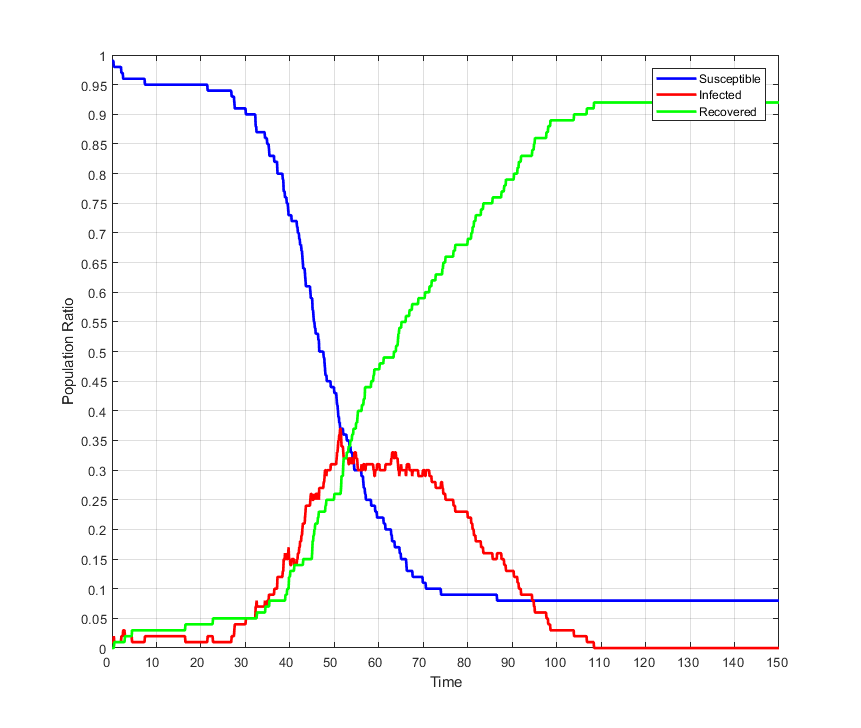
\includegraphics[width=1\textwidth, angle=0]{./fig/step2_yampa/SIR_100agents_150t_01dt.png}
			\caption{100 Agents, $\Delta t = 0.1$}
			\label{fig:sir_abs_approximating_01dt_100agents}
		\end{subfigure}
    	&
		\begin{subfigure}[b]{0.3\textwidth}
			\centering
			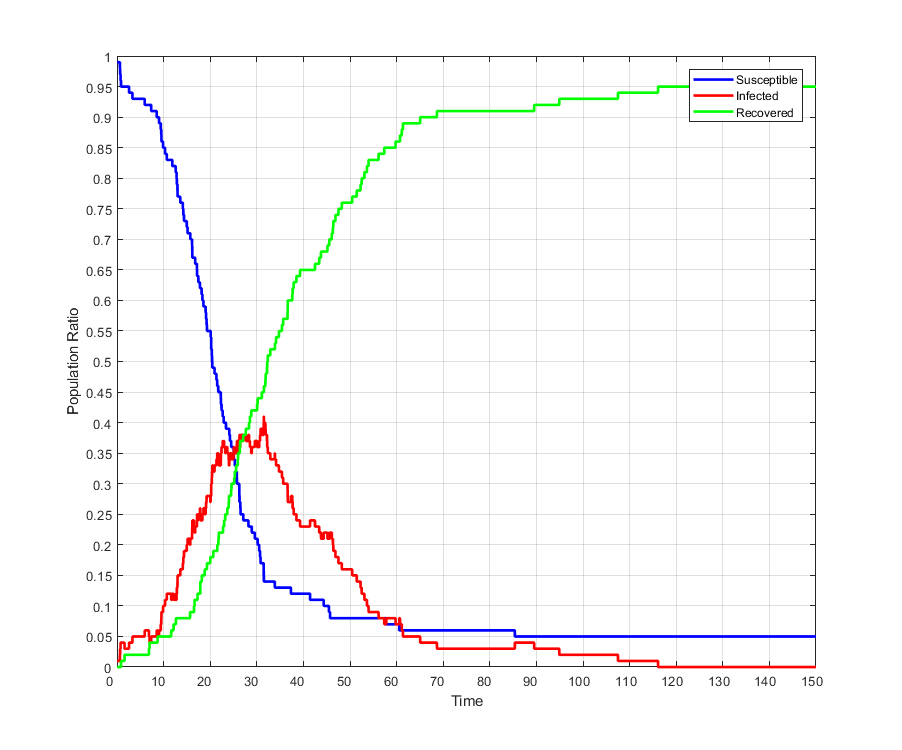
\includegraphics[width=1\textwidth, angle=0]{./fig/step2_yampa/SIR_100agents_150t_001dt.png}
			\caption{100 Agents, $\Delta t = 0.01$}
			\label{fig:sir_abs_approximating_001dt_500agents}
		\end{subfigure}
    	
    	\\
    	
		\begin{subfigure}[b]{0.3\textwidth}
			\centering
			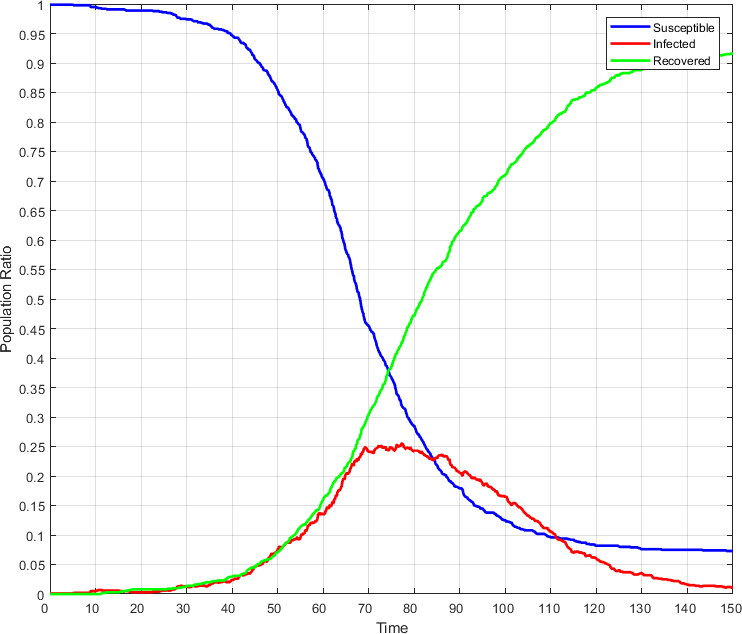
\includegraphics[width=1\textwidth, angle=0]{./fig/step2_yampa/SIR_1000agents_150t_01dt.png}
			\caption{1,000 Agents, $\Delta t = 0.1$}
			\label{fig:sir_abs_approximating_01dt_1000agents}
		\end{subfigure}
		& 
		\begin{subfigure}[b]{0.3\textwidth}
			\centering
			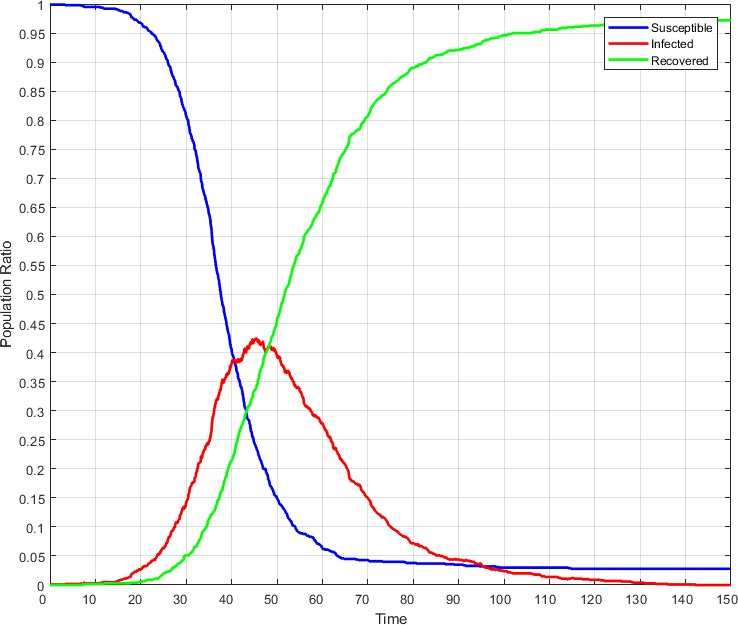
\includegraphics[width=1\textwidth, angle=0]{./fig/step2_yampa/SIR_1000agents_150t_001dt.png}
			\caption{1,000 Agents, $\Delta t = 0.01$}
			\label{fig:sir_abs_approximating_001dt_1000agents}
		\end{subfigure}
	\end{tabular}
	
	\caption{FRP simulation of SIR using agent-based approach. Population size of 100 and 1,000 with contact rate $\beta = \frac{1}{5}$, infection probability $\gamma = 0.05$, illness duration $\delta = 15$ with initially 1 infected agent. Simulation run for 150 time-steps with various $\Delta t$.} 
	\label{fig:sir_abs_dynamics_frp}
\end{center}
\end{figure}

Clearly by keeping the population size constant and just increasing the $\Delta t$ results in a closer approximation to the SD dynamics. Although the dynamics of Figure \ref{fig:sir_abs_approximating_001dt_1000agents} with 1000 agents and $\Delta t = 0.01$ look pretty close to SD, we are still not yet there. We would need to both decrease the sampling rate and increase the number of agents. Unfortunately at this point we are running into severe performance and memory problems because the whole system has to be sampled at an even finer $\Delta t$ whereas we only need to sample occasionally with higher frequency. A possible solution would be to implement super-sampling which would allow us to run the whole simulation with $\Delta t = 1.0$ and only sample the occasionally function with a much higher frequency. An approach would be to introduce a new function to Yampa which allows to super-sample other signal-functions. 

\begin{minted}[fontsize=\footnotesize]{haskell}
superSampling :: Int -> SF a b -> SF a [b]
\end{minted}

It evaluates \textit{sf} for \textit{n} times, each with $\Delta t = \frac{\Delta t}{n}$ and the same input argument \textit{a} for all \textit{n} evaluations. At time 0 no super-sampling is performed and just a single output of \textit{sf} is calculated. A list of \textit{b} is returned with length of \textit{n} containing the result of the \textit{n} evaluations of \textit{sf}. If 0 or less super samples are requested exactly one is calculated. We could then just wrap the occasionally function which would then generate a list of events. We have investigated super-sampling more in-depth but have to leave this due to lack of space.

\subsubsection{Discussion}
By moving on to FRP using Yampa we made a huge improvement in clarity, expressivity and robustness of our implementation. State is now implicitly encoded, depending on which signal-function is active. Also by using explicit time-semantics with \textit{occasionally} we can achieve extremely fine grained stochastics. Compared to drawing a random number of events we create only a single event or none at all. This requires to sample the system with a much smaller $\Delta t$: we are treating it as a truly continuous system, resulting in a hybrid SD/ABS approach.
Still we are not too happy about our approach as we feed back all agents states into every agent, something we want to omit in an agent-based simulation. We now move on to the next section in which we introduce a more general and much more controlled mechanism for feeding back agent-states. 

\subsection{Step III: Adding data-flow}
- getting rid of feeding all agent-states back into every agent, making data-flows explicit between agents, which is necessary because connections between agents are not fixed at compile time
- with occasionally we can achieve extremely fine grained stochastics as opposed to draw random number of events we create only a single event or not, this allows for a much smoother curve and is a real advantage: we are treating it as a continuous system

\subsection{Step IV: Generalising to Monadic Stream Functions}
- this allows us to add dynamic environments and agent transactions
- we need deterministic behaviour under all curcumstances, thus we cannot use IO or STM. for globally mutable state we use StateT
- also putting agentout into StateT monad composes now much better

\subsection{Step V: Adding an environment}
adding Environment: when in in/out its cumbersome, end up with n copies, pro-active Environment needs to be hacked in, have additional complexities
 
\subsection{Step VI: Adding agent transactions}
TX: running agents and with 0 dt is easy with bearriver.